\section{Gleichstromumrichter}
Ein Gleichstromumrichter dient zur änderung von: \textbf{Polarität, Spannung, Strom}.\newline
\subsection{Buck-Converter}
\begin{minipage}{0.75\linewidth}
    Tiefsetzsteller (Buck-Converter) $U_a < U_e  $\newline
    \textbf{Rechnung ohne C}\newline
    \[ \tau=\frac{L_1}{R_1} \qquad T_s=T_{on} + T_{off} \]
    \[ V_1 = i_L\cdot R_1+L_1\cdot\frac{\diff i_L}{\diff t} \qquad 0<t<T_{on} \]
    \[ 0 = i_L\cdot R_1+L_1\cdot\frac{\diff i_L}{\diff t} \qquad T_{on}<t<T_{s} \]    
    \[ i_L=\frac{V_1}{R_1}+ \frac{V_1}{R_1}\cdot \frac{e^{-\frac{T_{off}}{\tau}}-1}{1-e^{-\frac{T_{s}}{\tau}}}\cdot e^{-\frac{t}{\tau}} \qquad 0<t<T_{on}  \]
    \[ i_L=\frac{V_1}{R_1}\cdot \frac{1-e^{-\frac{T_{on}}{\tau}}}{1-e^{-\frac{T_{s}}{\tau}}}\cdot e^{-\frac{t-T_{on}}{\tau}} \qquad T_{on}<t<T_{s}  \]    
    \[ T_{on}=-\tau \cdot ln\frac{i_{Lmin}}{i_{Lmax}}= -\frac{L_1}{R_1}\cdot ln\frac{i_{Lmin}}{i_{Lmax}} \]    
    \[ T_{off}=-\tau \cdot ln\left(\frac{\frac{1}{i_{Lmax}}\cdot\frac{V_1}{R_1}-1}{\frac{1}{i_{Lmax}}\cdot \frac{V_1}{R_1}-e^{-\frac{T_off}{\tau}}}\right) \]
\end{minipage}
\begin{minipage}{0.25\linewidth}
    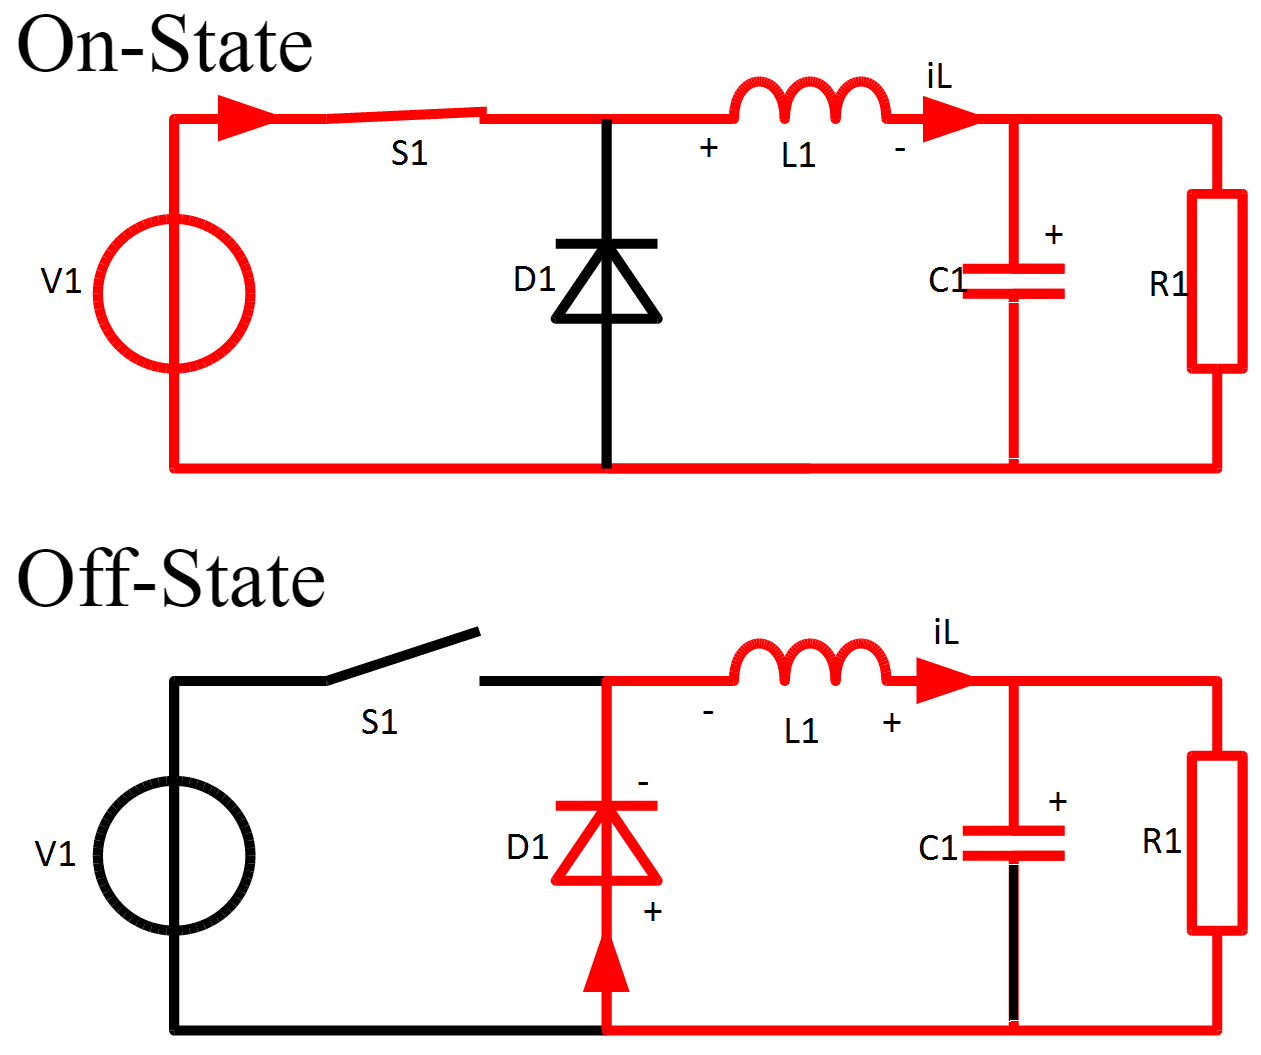
\includegraphics[width=\linewidth]{images/BuckOnOff}
    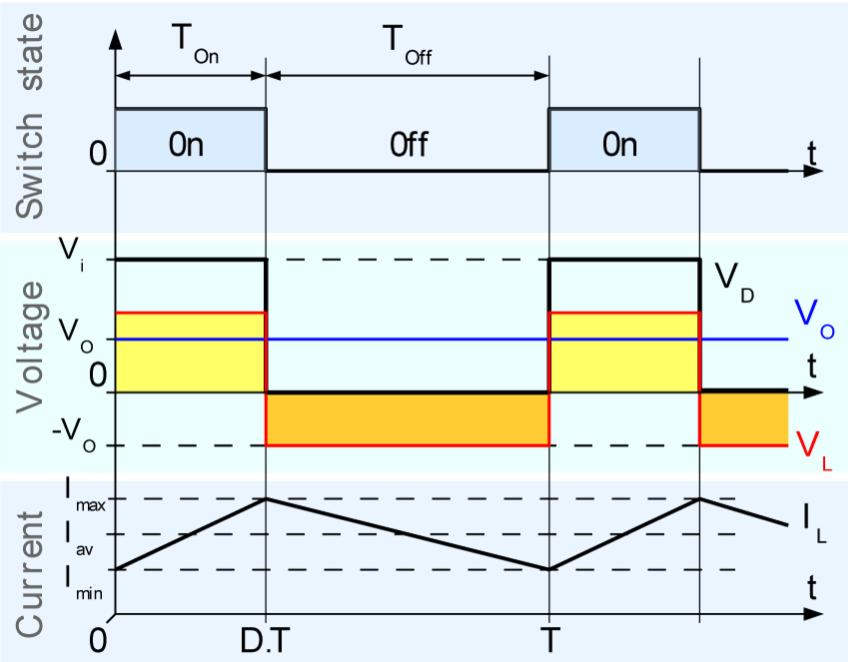
\includegraphics[width=\linewidth]{images/BuckSwitch}
\end{minipage}

\subsection{Boost-Converter}
\begin{minipage}{0.75\linewidth}
    Hochsetzsteller (Boost-Converter) $U_a > U_e  $\newline
    
\end{minipage}
\begin{minipage}{0.25\linewidth}
    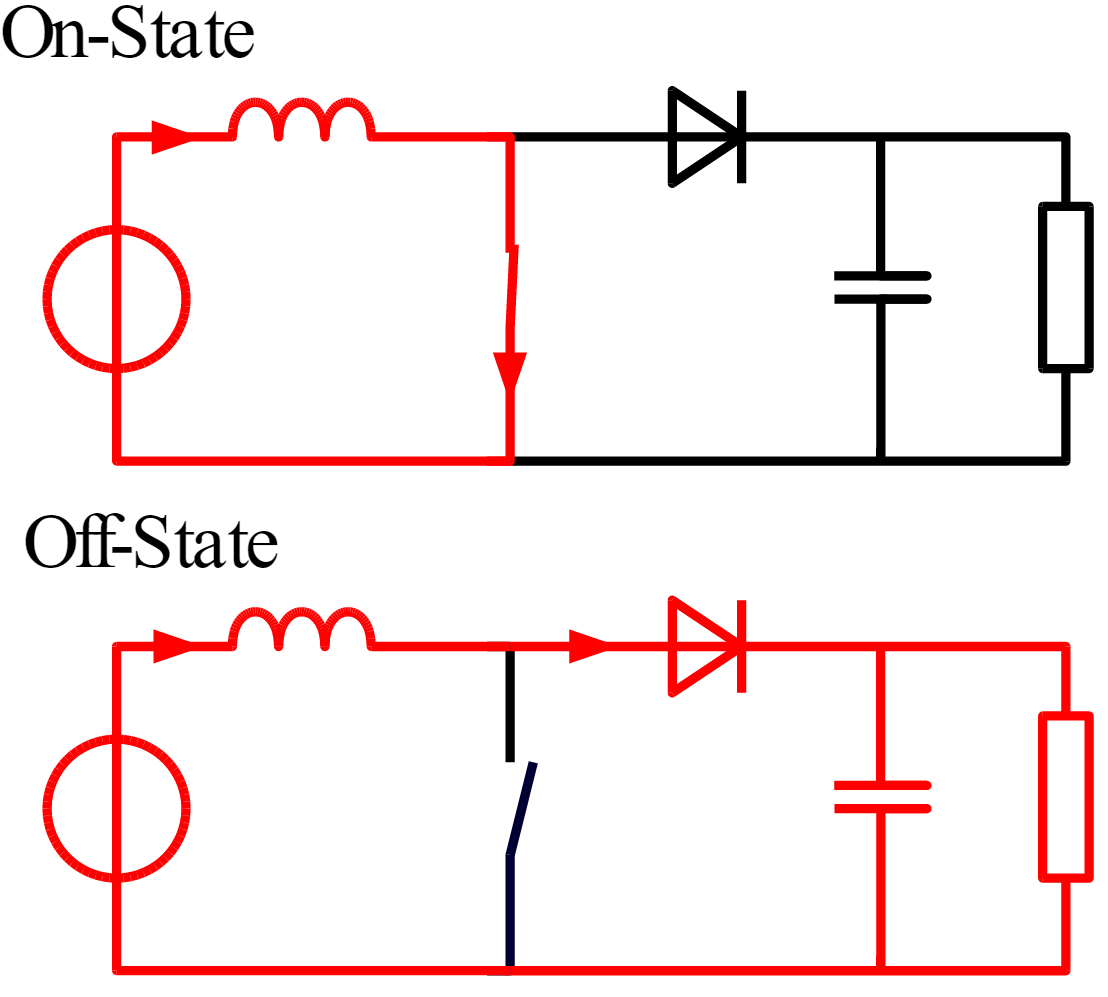
\includegraphics[width=\linewidth]{images/BoostOnOff}
    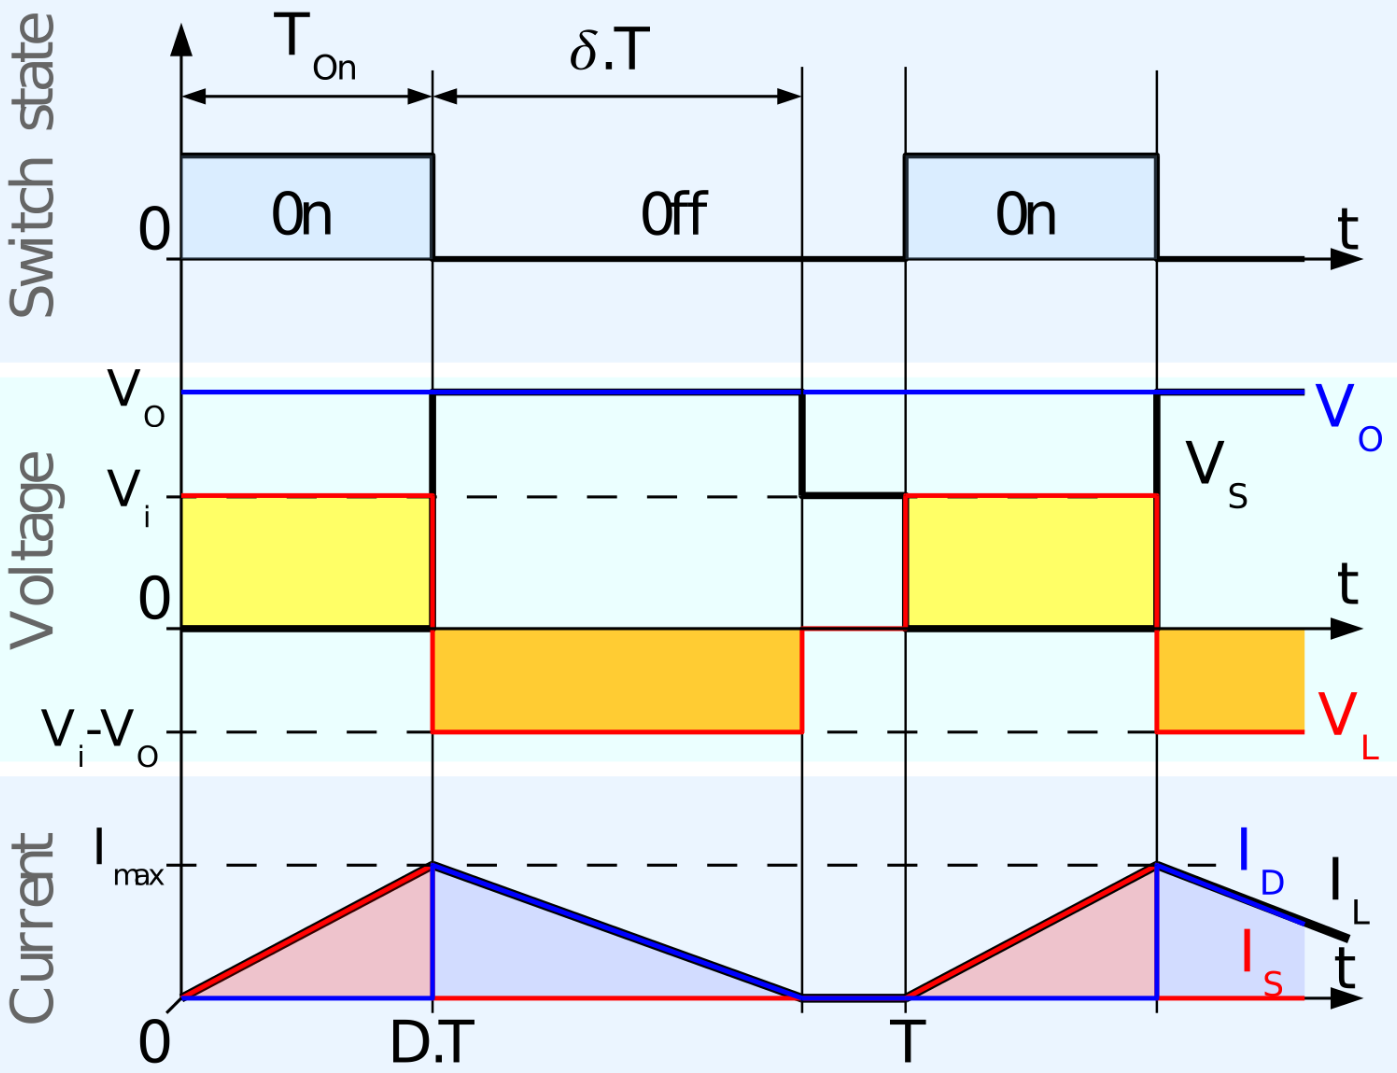
\includegraphics[width=\linewidth]{images/BoostSwitch}
\end{minipage}



\subsection{Inverse-Converter}
Inverswandler, Umkehrung der Polarität\newline

\subsection{Gleichstrom-Schalter/Steller}
\subsubsection{Gleichstrom-Schalter}

\subsubsection{Gleichstrom-Steller}
\clearpage